\documentclass[12pt]{article}

\usepackage{amsmath}
\usepackage{amssymb}
\usepackage[dvips]{graphicx}
\usepackage{eepic}
\usepackage{color}
\usepackage{wasysym} % \female \male
\usepackage[landscape,pdftex]{geometry}
\usepackage{fancyhdr}
\usepackage{wasysym} % for check symbol

\DeclareOption{bigsym}{\DeclareSymbolFont{largesymbols}{OMX}{psycm}{m}{n}}
\ProcessOptions

\setlength{\oddsidemargin}{-0.75in}
\setlength{\evensidemargin}{-0.75in}
\setlength{\topmargin}{-1in}
\setlength{\textheight}{7.75in}
\setlength{\textwidth}{10.5in}
\setlength{\footskip}{0in}
\setlength{\parindent}{0pt}
\setlength{\rightskip}{0pt plus 1fil} % makes ragged right

\renewcommand{\familydefault}{phv} % helvetica

% following: color
\definecolor{mybgcolor}{rgb}{0,0,0.3125}
\definecolor{myyellow}{rgb}{1,1,0.4}
\definecolor{myblue}{rgb}{0.4,0.8,1}
\definecolor{mypink}{rgb}{1,0.4,1}
\definecolor{myhotpink}{rgb}{1,0,0.5}
\definecolor{mywhite}{rgb}{1,1,1}

% following: B/W
%\definecolor{mybgcolor}{rgb}{1,1,1}
%\definecolor{myyellow}{rgb}{0,0,0}
%\definecolor{myblue}{rgb}{0,0,0}
%\definecolor{mypink}{rgb}{0,0,0}
%\definecolor{myhotpink}{rgb}{0,0,0}
%\definecolor{mywhite}{rgb}{0,0,0}

% header/footer layout
\pagestyle{fancy}
\lhead{} \chead{} \rhead{}
\lfoot{} \cfoot{} \rfoot{\color{myyellow} \thepage}
\renewcommand{\headrulewidth}{0pt}
\renewcommand{\footrulewidth}{0pt}

% font sizes
\newcommand{\superlarge}{\fontsize{60}{60} \selectfont}
\newcommand{\titlesize}{\fontsize{40}{50} \selectfont}
\newcommand{\headsize}{\fontsize{35}{35} \selectfont}
\newcommand{\textsize}{\fontsize{30}{35} \selectfont}
\newcommand{\smallsize}{\fontsize{25}{30} \selectfont}
\newcommand{\smallersize}{\fontsize{20}{25} \selectfont}
\newcommand{\smallestsize}{\fontsize{18}{22} \selectfont}
\newcommand{\evensmaller}{\fontsize{14}{18} \selectfont}
\newcommand{\lod}{\text{LOD}}
\newcommand{\bic}{\text{BIC}}
\newcommand{\rss}{\text{RSS}}
\newcommand{\var}{\text{var}}
\newcommand{\M}{\text{M}}
%\renewcommand{\log}{\text{log}}
%\renewcommand{\max}{\text{max}}



\pagecolor{mybgcolor}
\color{mywhite}

\begin{document}

\thispagestyle{empty}

\begin{center}
\titlesize \color{myyellow}

\vspace*{10mm}

{\headsize Identifying and correcting sample mix-ups \\
in high-dimensional genetic data}

\color{mypink}
\rule{10in}{1mm}
%\vspace{-10mm}

\vspace{10mm}

\textsize \color{myblue}
Karl W Broman
\vspace{5mm}

{\smallersize Department of Biostatistics \& Medical Informatics

University of Wisconsin -- Madison
\vspace{20mm}


\verb|www.biostat.wisc.edu/~kbroman| 
}

\end{center}


\newpage
\thispagestyle{empty}

\vspace*{-0.85in}

\centerline{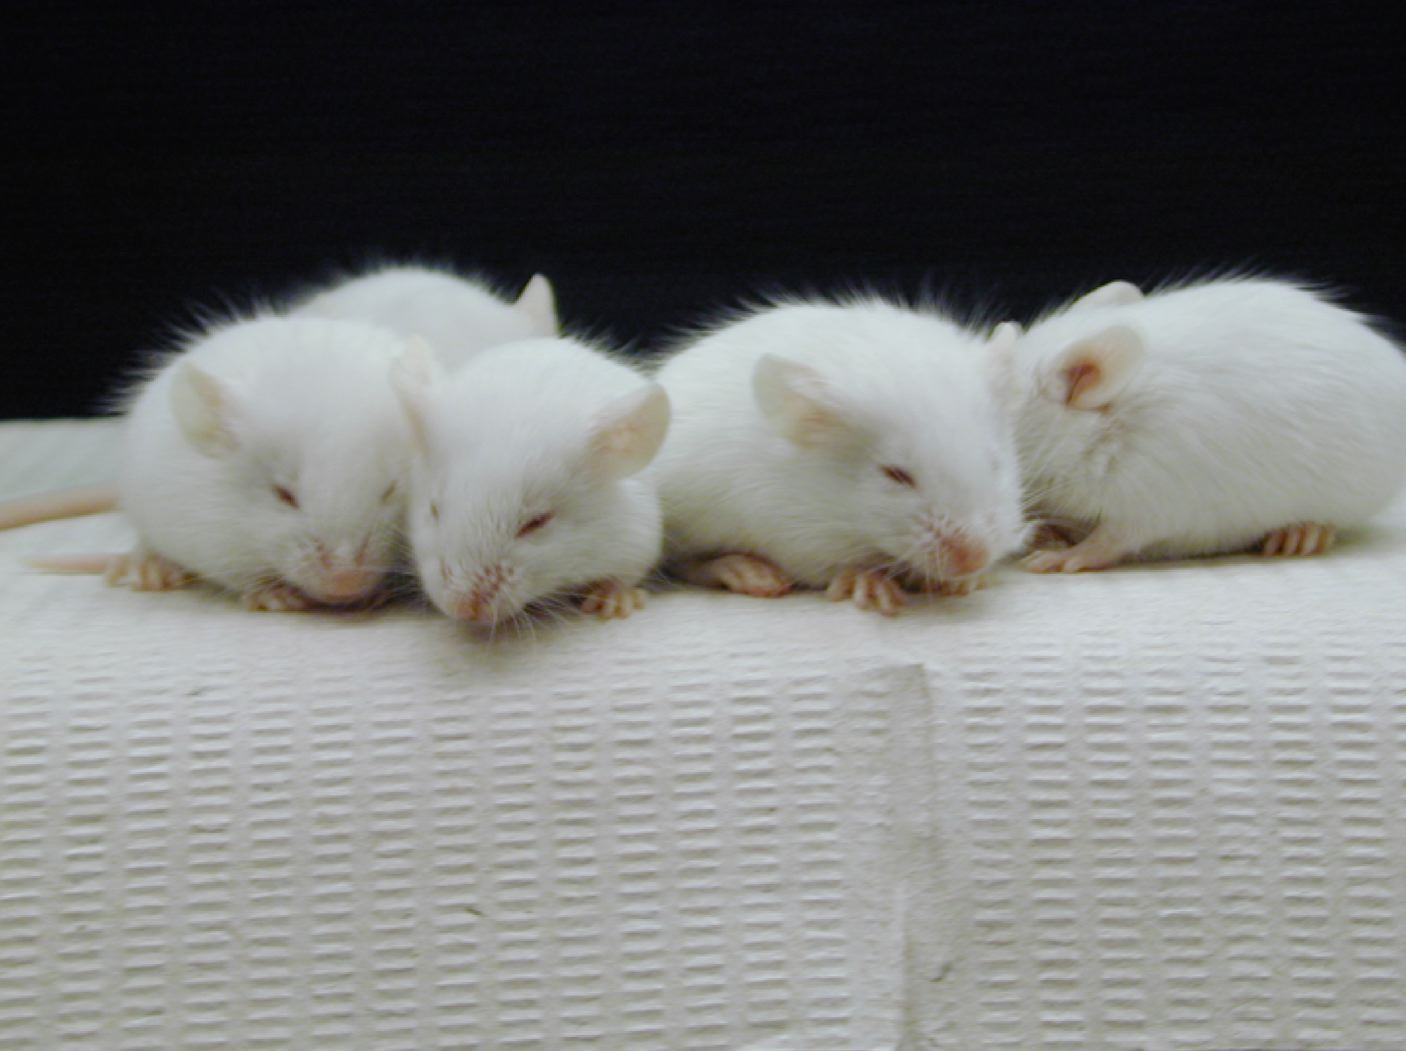
\includegraphics[height=9in]{Figs/inbredmice.jpg}}


\newpage

\headsize \color{myyellow}
\hfill \begin{minipage}{5.75in}
\centering
Human vs mouse
\end{minipage}

\vspace{3cm}

\centerline{
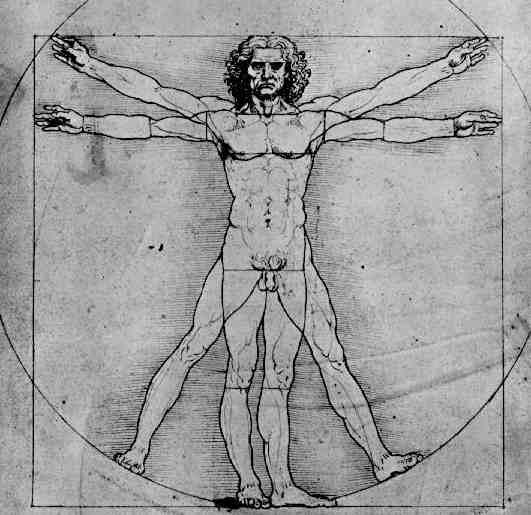
\includegraphics[height=5in]{Figs/da-vinci-man.jpg}
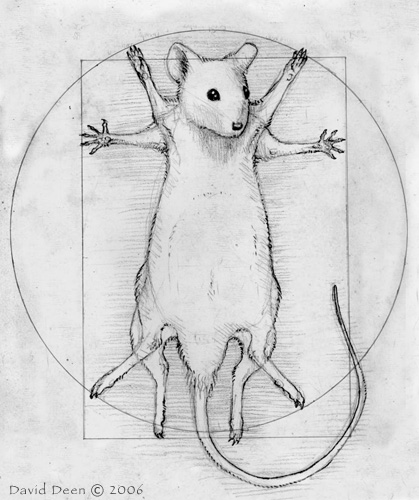
\includegraphics[height=5in]{Figs/vitruvian_mouse.jpg} 
}

{\color{myblue} \smallestsize \hfill \verb|www.daviddeen.com| \hspace*{11mm}}




\newpage

\headsize \color{myyellow}
\hfill 
\begin{minipage}{5.75in}
\centering
Attie project
\end{minipage}

\vspace{20mm}

\hfill \begin{minipage}{10in}

\smallsize
\color{mypink} 
$\sim$500 B6 $\times$ BTBR intercross mice, all ob/ob

\smallersize
\vspace{10mm}

\hfill \begin{minipage}{9in}
\color{mywhite}

Genotypes at 2057 SNPs (Affymetrix arrays)

\vspace{5mm}

Gene expression in six tissues (Agilent arrays)

{\color{myblue} \smallestsize
\hspace{20mm} adipose

\hspace{20mm} gastrocnemius muscle

\hspace{20mm}  hypothalamus

\hspace{20mm} pancreatic islets

\hspace{20mm} kidney

\hspace{20mm} liver
}
\vspace{5mm}

Numerous clinical phenotypes 

{\color{myblue}  \smallestsize
\hspace{20mm} (e.g., body weight, insulin and glucose
levels)
}

%\vspace{5mm}
%
%Considerable brain power
%
%{\color{myblue} \smallestsize
%\hspace{20mm} Alan Attie, Karl Broman, Aimee Teo Broman, Danielle Greenawalt, 
%
%\hspace{20mm} Mark
%Keller, Christina Kendziorski, Amit Kulkarni, Eric Schadt, 
%
%\hspace{20mm} Brian
%Yandell, \dots}



\end{minipage}

\end{minipage}

\newpage

\headsize \color{myyellow}
\hfill \begin{minipage}{5.75in}
\centering
Sex and the X chr
\end{minipage}

\vfill

\begin{minipage}[t]{5.5in}
\vspace*{0mm}

\includegraphics{Figs/xchr_fig.pdf}
\end{minipage}
\hfill
\begin{minipage}[t]{4.8in}
\vspace*{35mm}

\smallersize
\color{mywhite}



\begin{tabular}{ll}
F$_{\text{2}}$ females: & {\color{myblue} R/R or B/R} \\[18pt]
F$_{\text{2}}$ males: & {\color{myblue} hemizygous B or R}
\end{tabular}

\end{minipage}

\newpage


\headsize \color{myyellow}
\hfill \begin{minipage}{5.75in}
\centering
Genotype mix-ups
\end{minipage}

\vfill

\centerline{\includegraphics{Figs/plate_errors.pdf}}

\newpage

\headsize \color{myyellow}
\hfill \begin{minipage}{5.75in}
\centering
Sex and the X chr
\end{minipage}

\vfill

\begin{minipage}[t]{5.5in}
\vspace*{0mm}

\includegraphics{Figs/xchr_fig.pdf}
\end{minipage}
\hfill
\begin{minipage}[t]{4.8in}
\vspace*{35mm}

\smallersize
\color{mywhite}



\begin{tabular}{ll}
F$_{\text{2}}$ females: & {\color{myblue} R/R or B/R} \\[18pt]
F$_{\text{2}}$ males: & {\color{myblue} hemizygous B or R}
\end{tabular}

\end{minipage}

\newpage



\headsize \color{myyellow}
\hfill \begin{minipage}{5.75in}
\centering
Strong eQTL
\end{minipage}

\vfill

\centerline{\includegraphics{Figs/eqtl_lod_1.pdf}}

\newpage

\headsize \color{myyellow}
\hfill \begin{minipage}{5.75in}
\centering
Strong eQTL
\end{minipage}

\vfill

\centerline{\includegraphics{Figs/eqtl_lod_2.pdf}}

\newpage



\headsize \color{myyellow}
\hfill \begin{minipage}{5.75in}
\centering
E vs G
\end{minipage}

\vfill

\centerline{\includegraphics{Figs/gve1a.pdf}}

\newpage


\headsize \color{myyellow}
\hfill \begin{minipage}{5.75in}
\centering
E vs G
\end{minipage}

\vfill

\centerline{\includegraphics{Figs/gve1b.pdf}}

\newpage


\headsize \color{myyellow}
\hfill \begin{minipage}{5.75in}
\centering
kNN classifier
\end{minipage}

\vfill

\centerline{\includegraphics{Figs/gve1c.pdf}}

\newpage


\headsize \color{myyellow}
\hfill \begin{minipage}{5.75in}
\centering
E vs G
\end{minipage}

\vfill

\centerline{\includegraphics{Figs/gve3a.pdf}}

\newpage


\headsize \color{myyellow}
\hfill \begin{minipage}{5.75in}
\centering
E vs G
\end{minipage}

\vfill

\centerline{\includegraphics{Figs/gve3b.pdf}}

\newpage

\headsize \color{myyellow}
\hfill \begin{minipage}{5.75in}
\centering
E vs G
\end{minipage}

\vfill

\centerline{\includegraphics{Figs/gve2a.pdf}}

\newpage


\headsize \color{myyellow}
\hfill \begin{minipage}{5.75in}
\centering
E vs G
\end{minipage}

\vfill

\centerline{\includegraphics{Figs/gve2b.pdf}}





\newpage


\headsize \color{myyellow}
\hfill \begin{minipage}{5.75in}
\centering
Basic scheme
\end{minipage}

\vfill

\centerline{\includegraphics{Figs/gve_scheme_1.pdf}}

\newpage

\headsize \color{myyellow}
\hfill \begin{minipage}{5.75in}
\centering
Basic scheme
\end{minipage}

\vfill

\centerline{\includegraphics{Figs/gve_scheme_2.pdf}}

\newpage

\headsize \color{myyellow}
\hfill \begin{minipage}{5.75in}
\centering
Basic scheme
\end{minipage}

\vfill

\centerline{\includegraphics{Figs/gve_scheme_3.pdf}}

\newpage

\headsize \color{myyellow}
\hfill \begin{minipage}{5.75in}
\centering
Basic scheme
\end{minipage}

\vfill

\centerline{\includegraphics{Figs/gve_scheme_4.pdf}}

\newpage

\headsize \color{myyellow}
\hfill \begin{minipage}{5.75in}
\centering
Prop'n mismatches
\end{minipage}

\vfill

\centerline{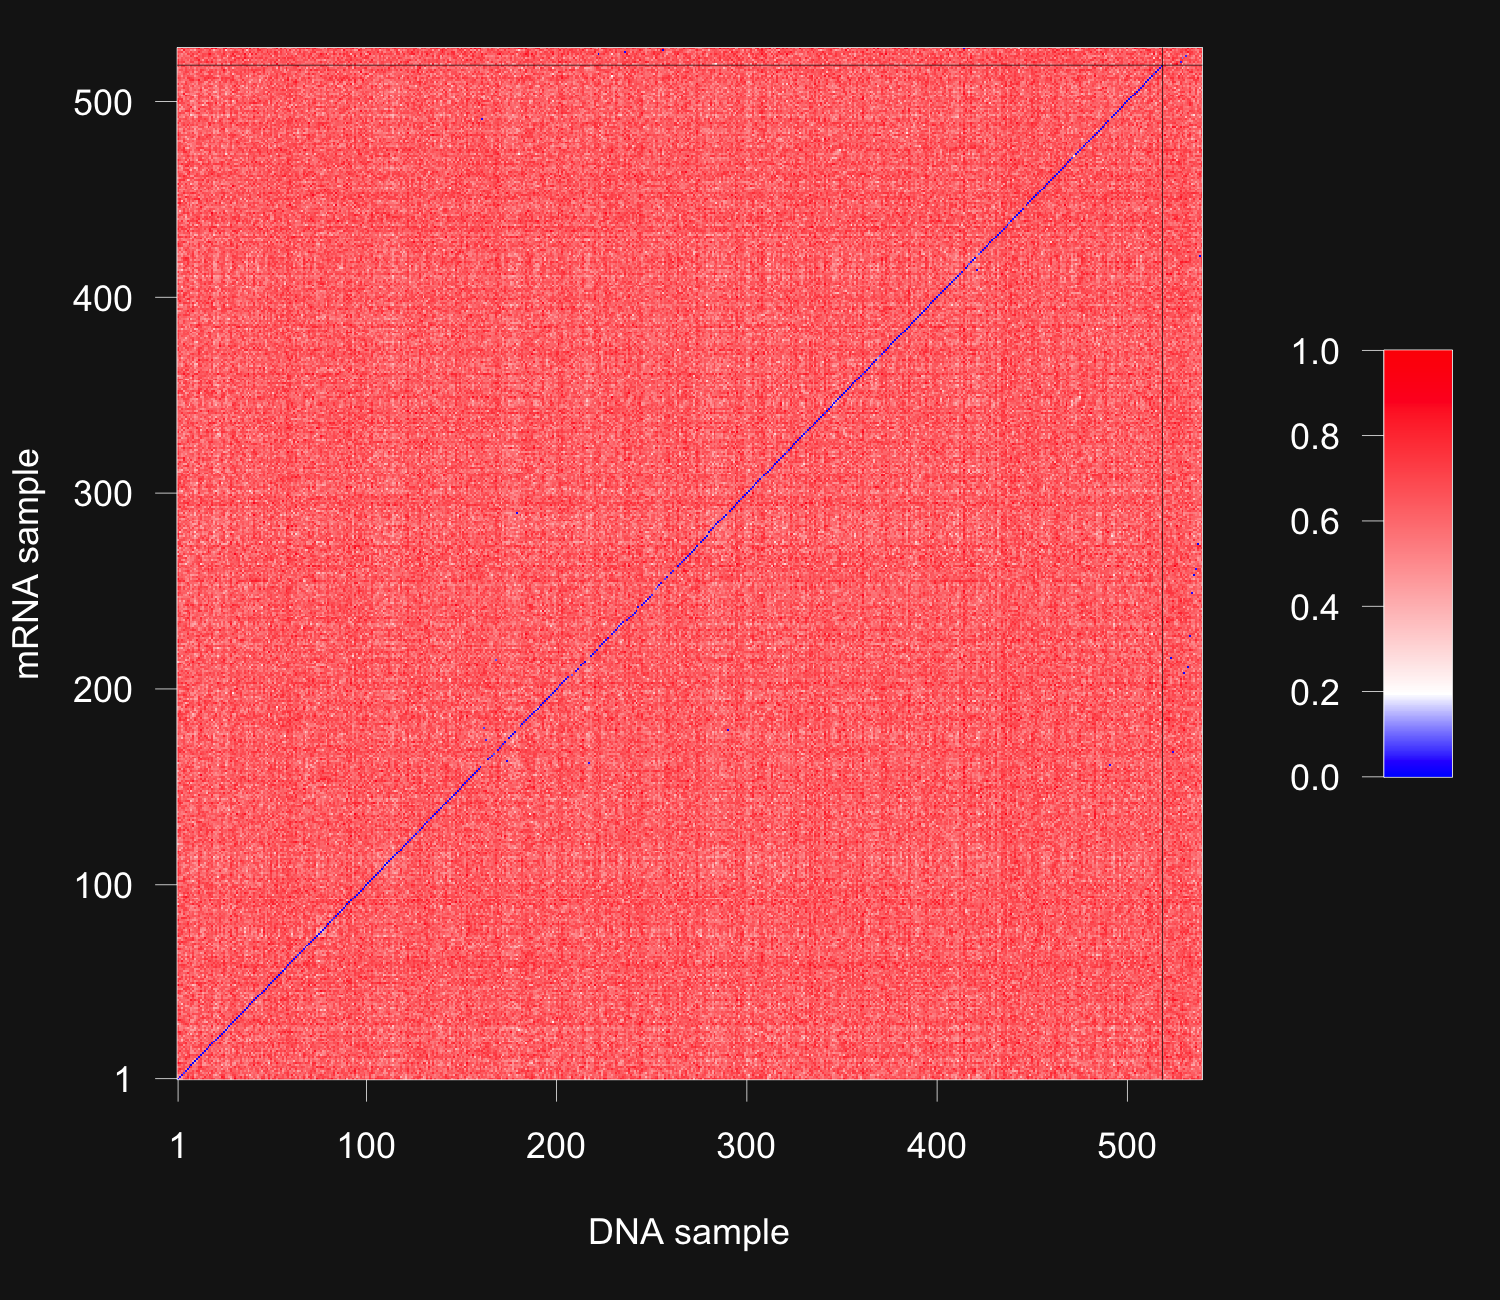
\includegraphics[height=6.5in]{Figs/distmatall.png}}

\newpage



\headsize \color{myyellow}
\hfill \begin{minipage}{5.75in}
\centering
Prop'n mismatches
\end{minipage}

\vfill

\centerline{\includegraphics{Figs/distmat001.pdf}}

\newpage




\headsize \color{myyellow}
\hfill \begin{minipage}{5.75in}
\centering
Prop'n mismatches
\end{minipage}

\vfill

\centerline{\includegraphics{Figs/distmat201.pdf}}

\newpage




%\headsize \color{myyellow}
%\hfill \begin{minipage}{5.75in}
%\centering
%The diagonal
%\end{minipage}
%
%\vfill
%
%\centerline{\includegraphics{Figs/distmatdiag.pdf}}
%
%\newpage




\headsize \color{myyellow}
\hfill \begin{minipage}{5.75in}
\centering
Prop'n mismatches
\end{minipage}

\vfill

\centerline{\includegraphics{Figs/gve_dist.pdf}}

\newpage


\headsize \color{myyellow}
\hfill \begin{minipage}{5.75in}
\centering
Decisions
\end{minipage}

\vfill

\centerline{\includegraphics{Figs/gve_dist_byrow_left.pdf}}

\newpage


\headsize \color{myyellow}
\hfill \begin{minipage}{5.75in}
\centering
Genotype mix-ups
\end{minipage}

\vfill

\centerline{\includegraphics{Figs/plate_errors.pdf}}

\newpage


\headsize \color{myyellow}
\hfill \begin{minipage}{5.75in}
\centering
Plate 1631
\end{minipage}

\vfill

\centerline{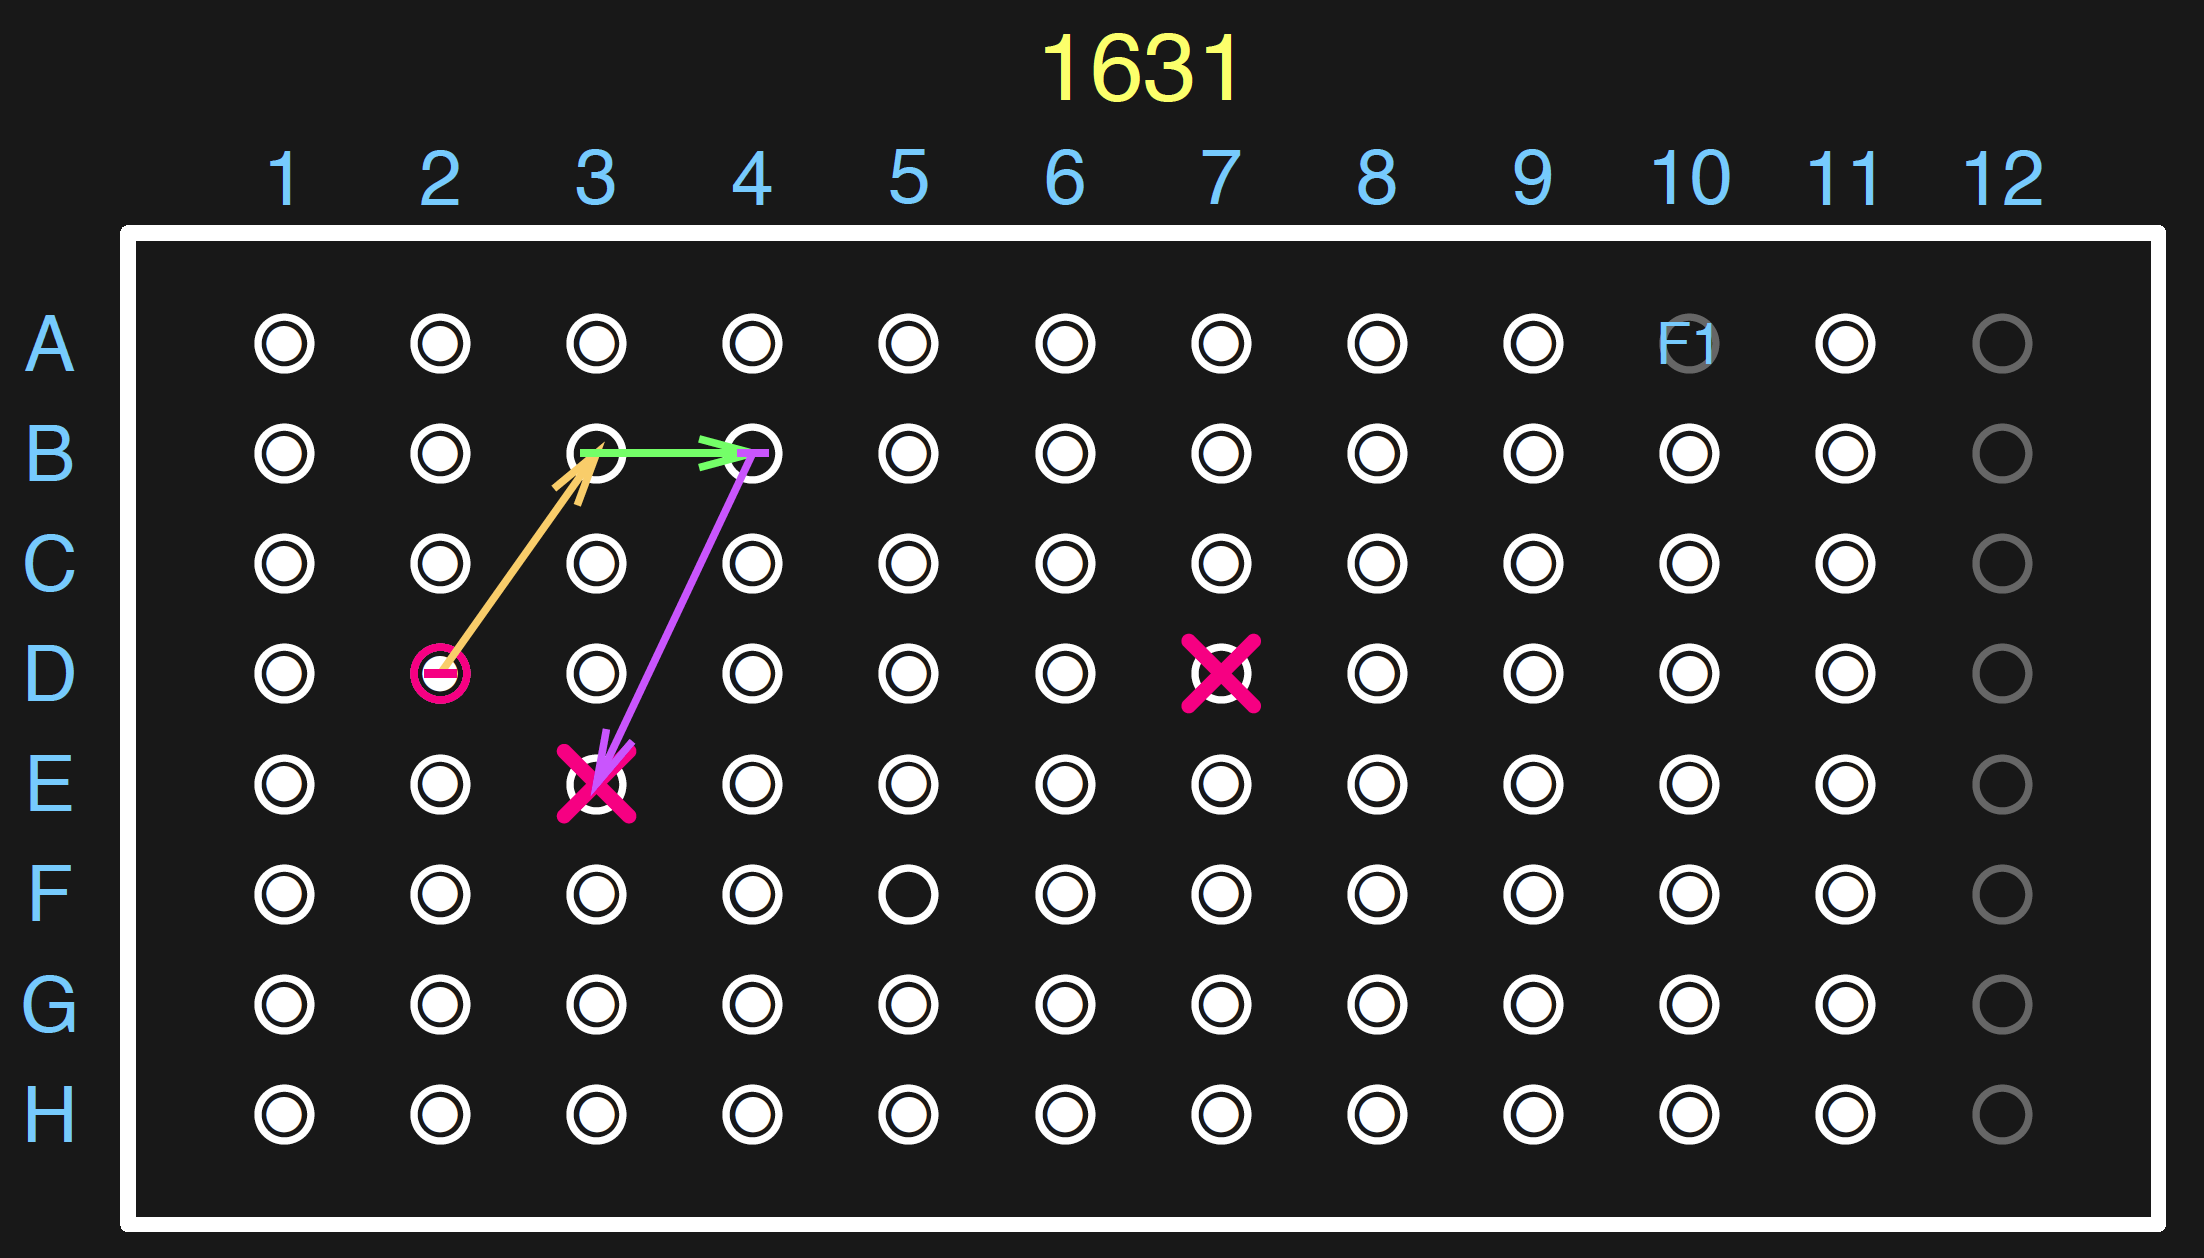
\includegraphics[width=10in]{Figs/plate_errors_1631.pdf}}

\newpage


\headsize \color{myyellow}
\hfill \begin{minipage}{5.75in}
\centering
Plates 1632 and 1630
\end{minipage}

\vfill

\centerline{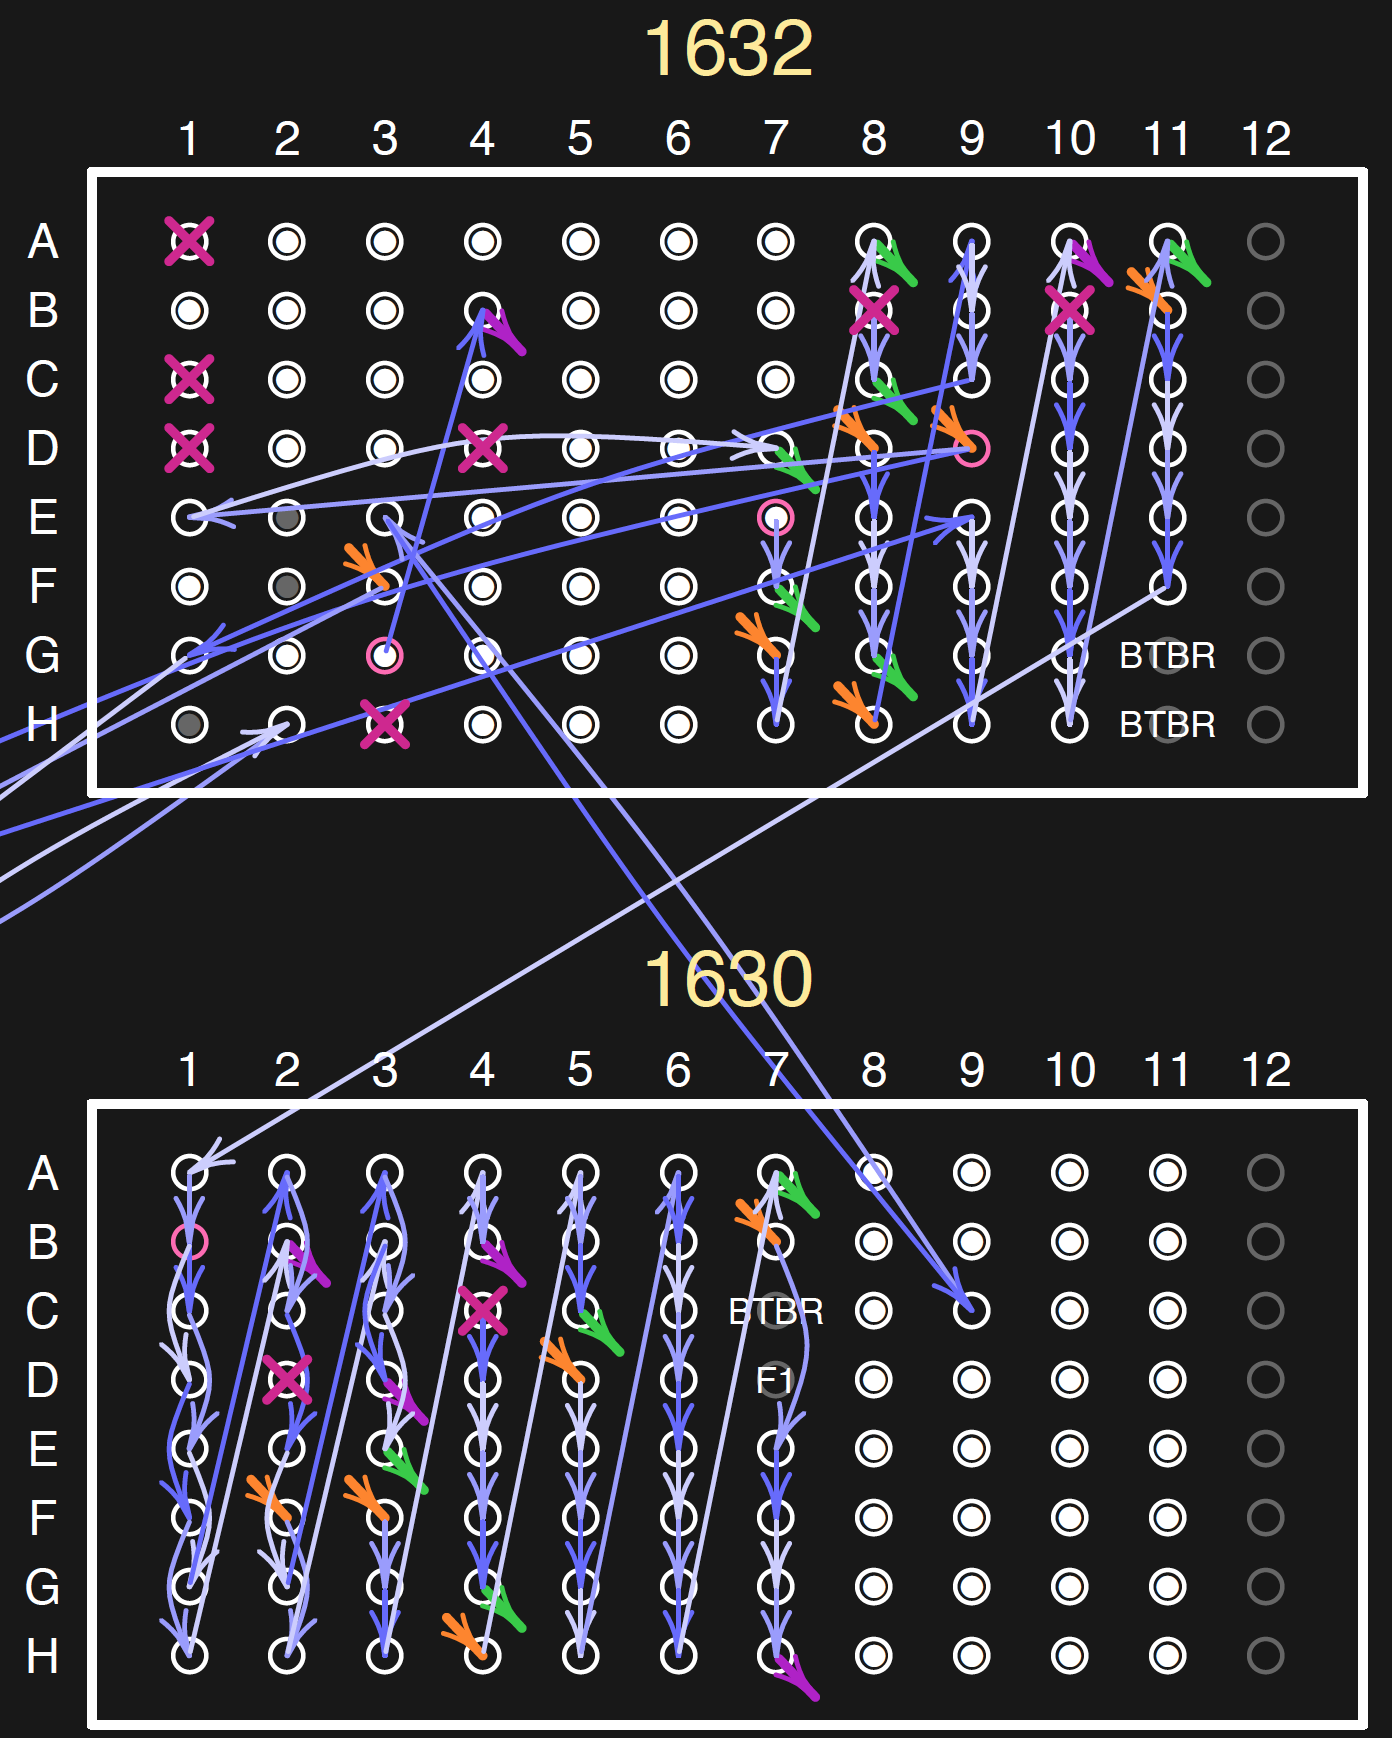
\includegraphics[height=6.5in]{Figs/plate_errors_1632_n_1630.pdf}}

\newpage


\headsize \color{myyellow}
\hfill \begin{minipage}{5.75in}
\centering
Plate 1630
\end{minipage}

\vfill

\centerline{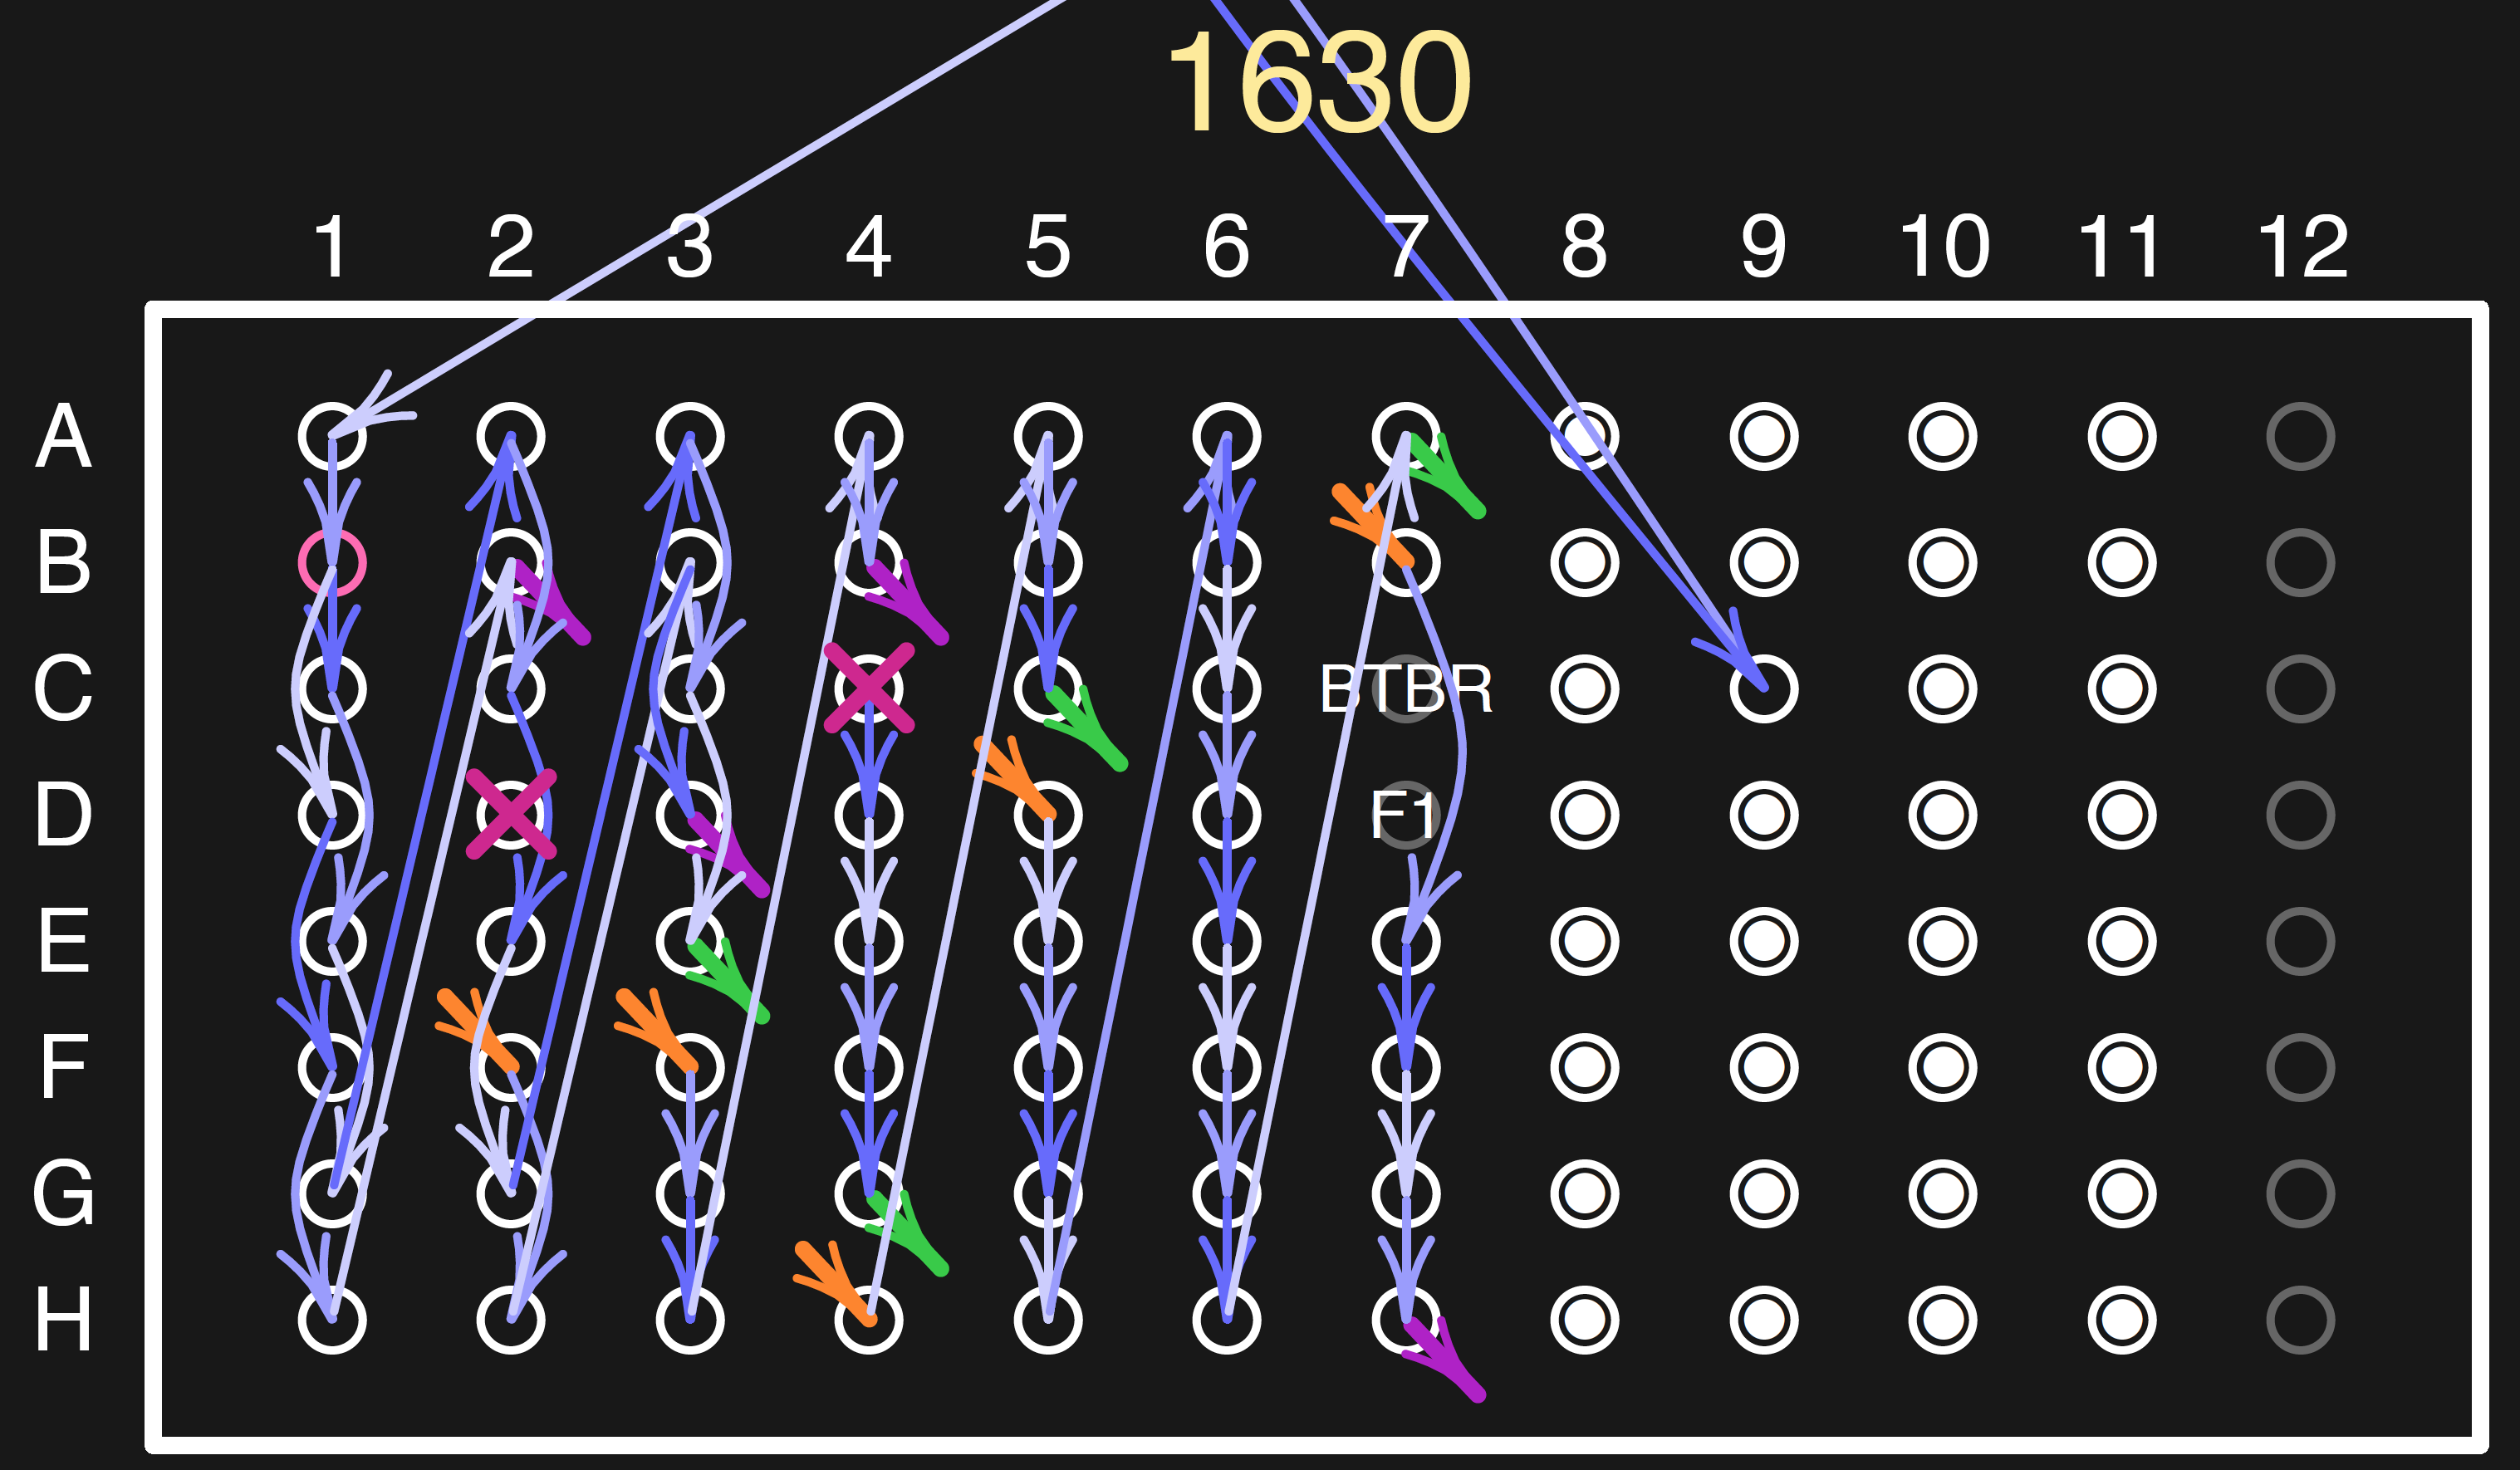
\includegraphics[width=10in]{Figs/plate_errors_1630.pdf}}

\newpage


\headsize \color{myyellow}
\hfill \begin{minipage}{5.75in}
\centering
E vs E
\end{minipage}

\vfill

\centerline{\includegraphics{Figs/eve_1.pdf}}

\newpage

\headsize \color{myyellow}
\hfill \begin{minipage}{5.75in}
\centering
E vs E
\end{minipage}

\vfill

\centerline{\includegraphics{Figs/eve_2.pdf}}

\newpage

\headsize \color{myyellow}
\hfill \begin{minipage}{5.75in}
\centering
E vs E
\end{minipage}

\vfill

\centerline{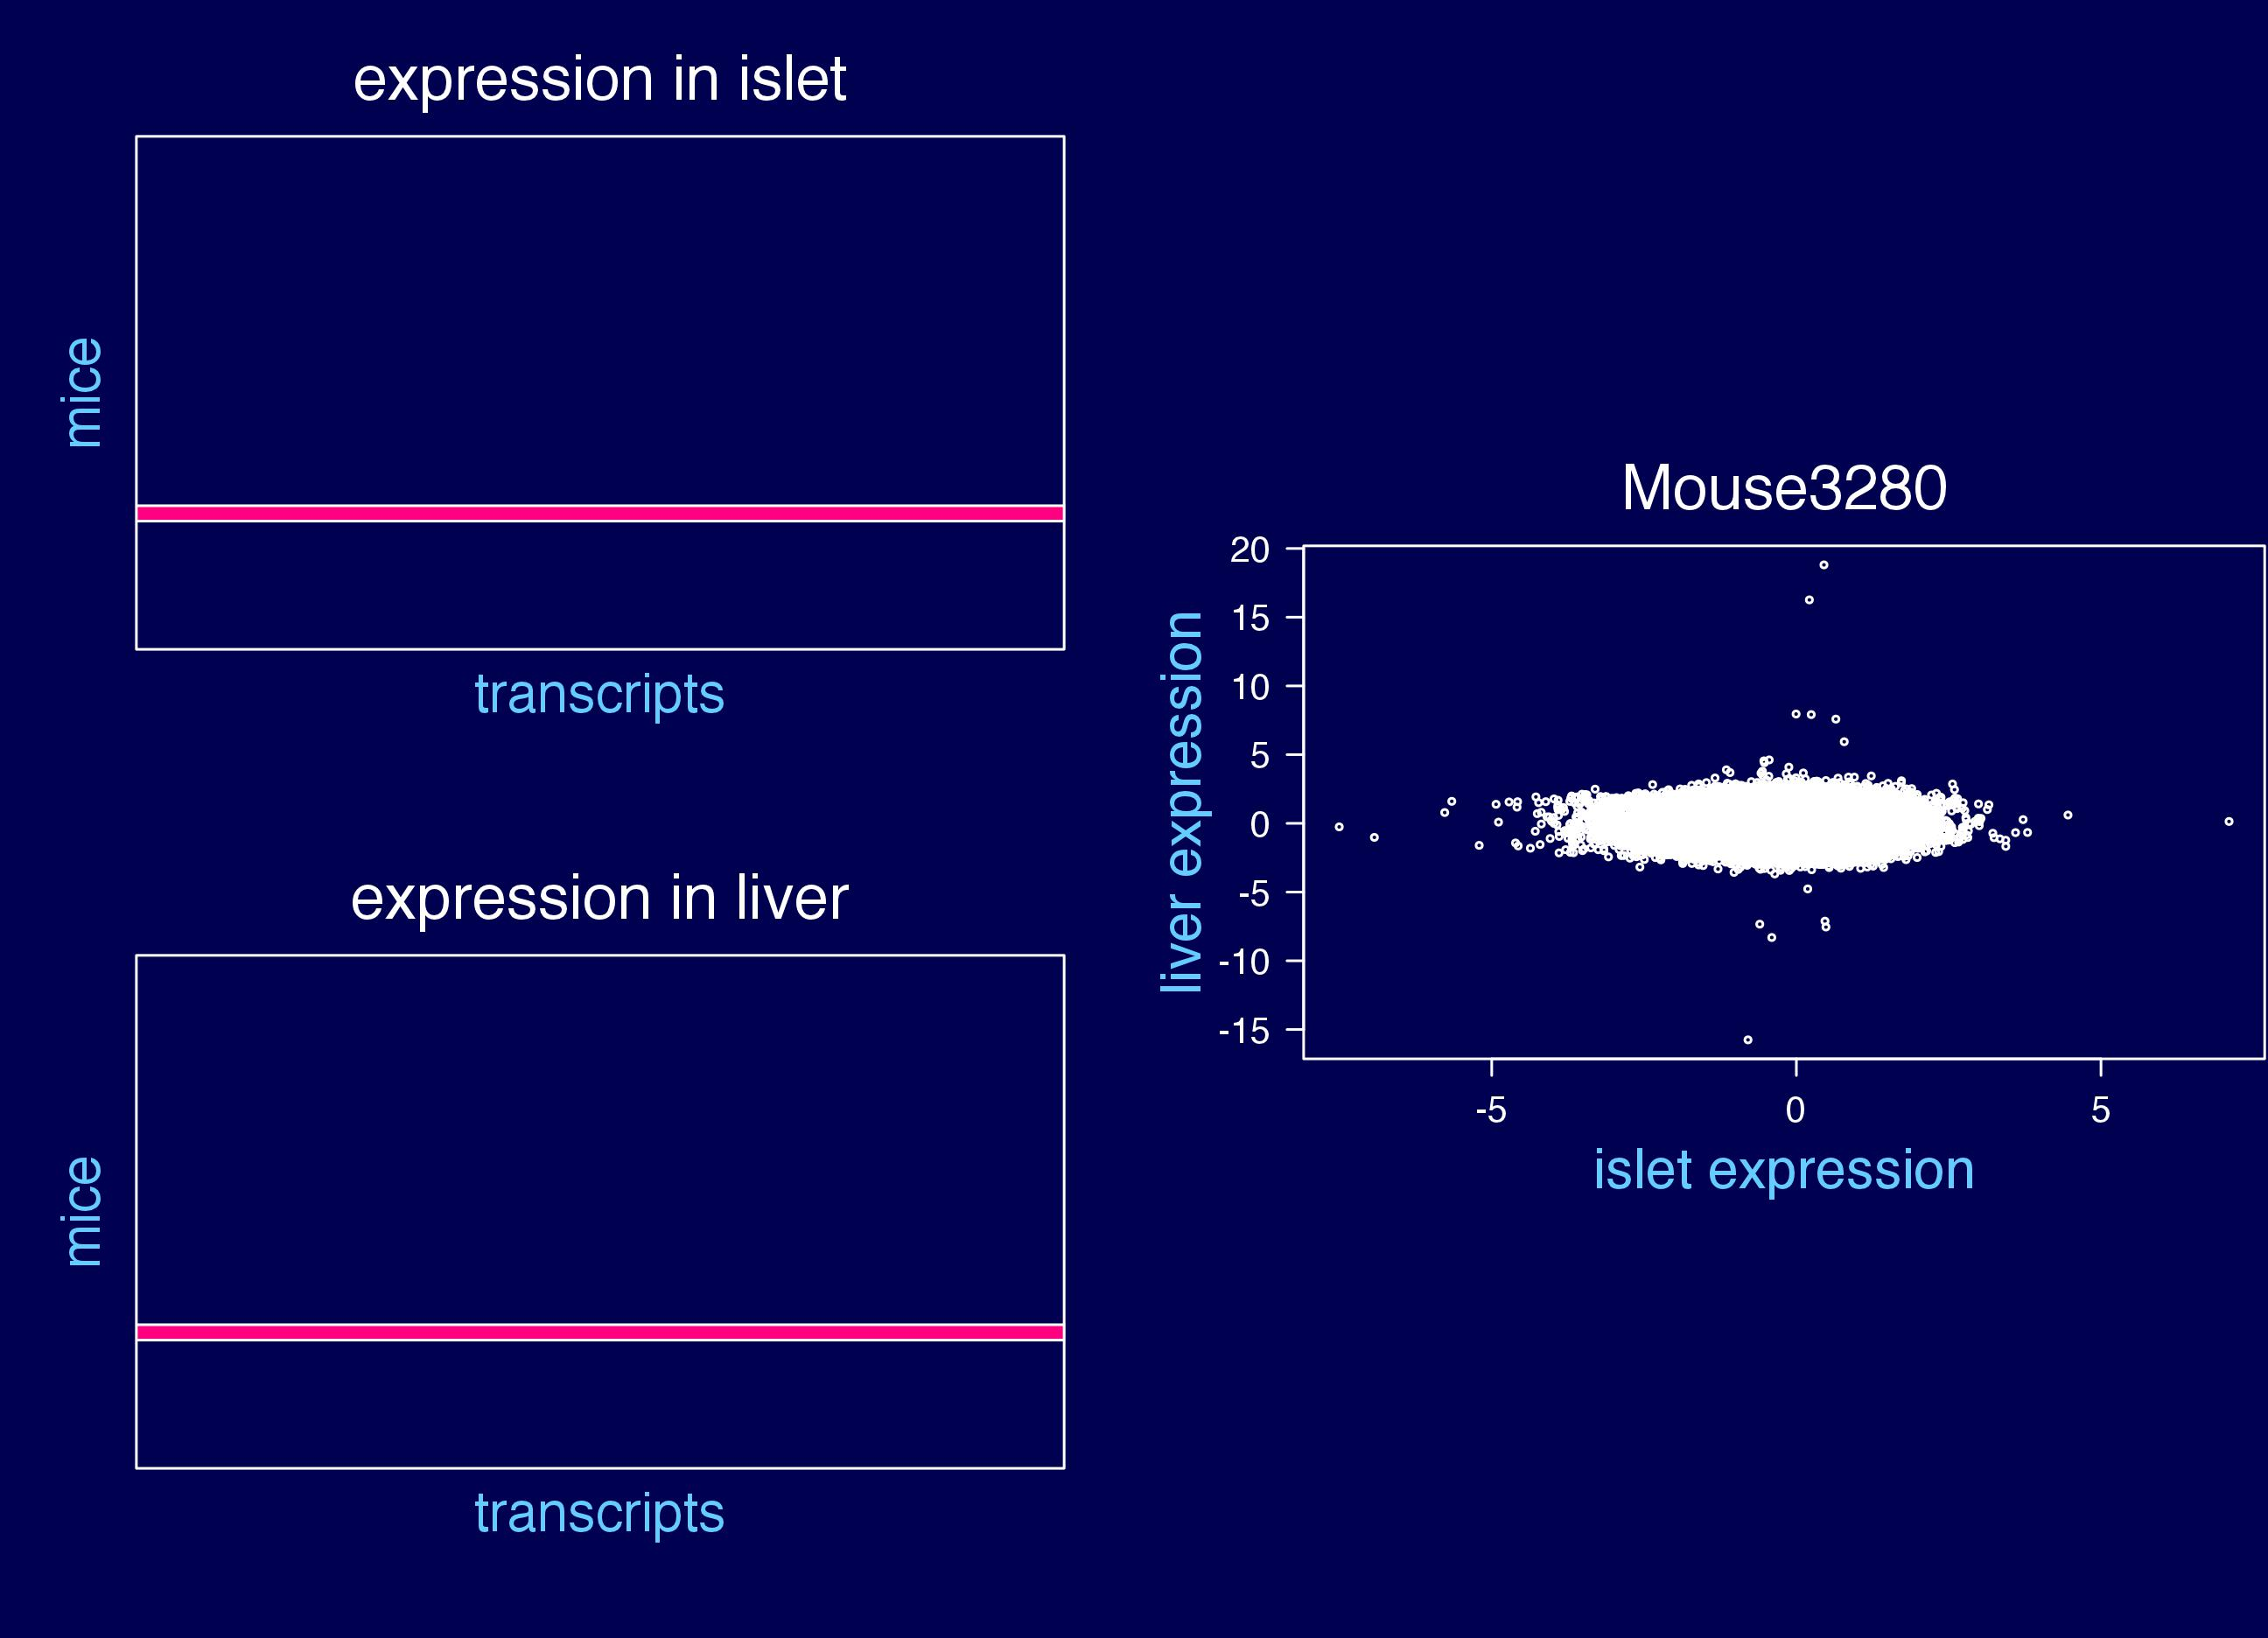
\includegraphics{Figs/eve_3.jpg}}


\newpage

\headsize \color{myyellow}
\hfill \begin{minipage}{5.75in}
\centering
E vs E
\end{minipage}

\vfill

\centerline{\includegraphics{Figs/eve_3b.pdf}}


\newpage

\headsize \color{myyellow}
\hfill \begin{minipage}{5.75in}
\centering
E vs E
\end{minipage}

\vfill

\centerline{\includegraphics{Figs/eve_3c.pdf}}


\newpage

\headsize \color{myyellow}
\hfill \begin{minipage}{5.75in}
\centering
E vs E
\end{minipage}

\vfill

\centerline{\includegraphics{Figs/eve_3d.pdf}}


\newpage

\headsize \color{myyellow}
\hfill \begin{minipage}{5.75in}
\centering
E vs E
\end{minipage}

\vfill

\centerline{\includegraphics{Figs/eve_4.pdf}}


\newpage

\headsize \color{myyellow}
\hfill \begin{minipage}{5.75in}
\centering
E vs E
\end{minipage}

\vfill

\centerline{\includegraphics{Figs/eve_5.pdf}}



\newpage

\headsize \color{myyellow}
\hfill \begin{minipage}{5.75in}
\centering
E vs E
\end{minipage}

\vfill

\centerline{\includegraphics{Figs/eve_6.pdf}}



\newpage

\headsize \color{myyellow}
\hfill \begin{minipage}{5.75in}
\centering
E vs E
\end{minipage}

\vfill

\centerline{\includegraphics{Figs/eve_7.pdf}}


\newpage

\headsize \color{myyellow}
\hfill \begin{minipage}{5.75in}
\centering
E vs E
\end{minipage}

\vfill

\centerline{\includegraphics{Figs/eve_8.pdf}}


\newpage

\headsize \color{myyellow}
\hfill \begin{minipage}{5.75in}
\centering
E vs E
\end{minipage}

\vfill

\centerline{\includegraphics{Figs/eve_9.pdf}}


\newpage

\headsize \color{myyellow}
\hfill \begin{minipage}{5.75in}
\centering
E vs E
\end{minipage}

\vfill

\centerline{\includegraphics{Figs/eve_10.pdf}}


\newpage

\headsize \color{myyellow}
\hfill \begin{minipage}{5.75in}
\centering
E vs E
\end{minipage}

\vfill

\centerline{\includegraphics{Figs/eve_11.pdf}}




\newpage


\headsize \color{myyellow}
\hfill \begin{minipage}{5.75in}
\centering
Insulin QTL
\end{minipage}

\vfill

\centerline{\includegraphics{Figs/insulin_lod.pdf}}


\newpage

\headsize \color{myyellow}
\hfill \begin{minipage}{5.75in}
\centering
Strong eQTL
\end{minipage}

\vfill

\centerline{\includegraphics{Figs/eqtl_lod_3.pdf}}



\newpage

\headsize \color{myyellow}
\hfill \begin{minipage}{5.75in}
\centering
Summary
\end{minipage}

\vspace{3cm} \color{mywhite} \smallersize

\hfill \begin{minipage}{10in}

\begin{itemize}
\itemsep24pt

\item Sample mix-ups happen

%\hspace{5mm} {\smallestsize \color{myblue} (But I bet mine are worse than
%  yours!)}


\item With eQTL data, we can both identify and {\color{mypink}
  correct} mix-ups

\item There is great value in having expression on multiple tissues

\item The general idea here has wide application for high-throughput data

\item Related work:

\smallestsize \color{myblue}
\begin{itemize}
\item Westra et al. (2011) Bioinformatics 27:2104--2111
\item Schadt et al. (2012) Nat Genet 44:603--608
\item Ekstr{\o}m and Feenstra (2012) Stat Appl Genet Mol Biol
  3:Article 13
\item Lynch et al. (2012) PLoS ONE 7:e41815
\end{itemize}

\end{itemize}
\end{minipage}



\newpage

\headsize \color{myyellow}
\hfill \begin{minipage}{5.75in}
\centering
Lessons
\end{minipage}

\vspace{20mm} \color{mywhite} \smallersize

\hfill \begin{minipage}{10in}

\begin{itemize}
\itemsep24pt

\item Don't fully trust anyone
{\smallestsize \color{myblue}
\begin{itemize}
\item Including yourself
\end{itemize} }

\item Make lots of plots
{\smallestsize \color{myblue}
\begin{itemize}
\item Don't rely on summary statistics, like LOD scores
\item Look at responses on the original scale
\end{itemize} }

\item Follow up all aberrations

\item Take your time with data cleaning
{\smallestsize \color{myblue}
\begin{itemize}
\item A month, two months, a year?
\end{itemize} }

\item Have a system for keeping track of everything
{\smallestsize \color{myblue}
\begin{itemize}
\item Files, versions of files, analyses, \dots
\item Like a lab notebook
\end{itemize} }



\end{itemize}
\end{minipage}


\newpage

\headsize \color{myyellow}
\hfill \begin{minipage}{5.75in}
\centering
E vs G

{\smallersize \color{mywhite} transformed scale}
\end{minipage}

\vfill

\centerline{\includegraphics{Figs/gve1a_nqrank.pdf}}

\newpage

\headsize \color{myyellow}
\hfill \begin{minipage}{5.75in}
\centering
E vs G

{\smallersize \color{mywhite} original scale}
\end{minipage}

\vfill

\centerline{\includegraphics{Figs/gve1a.pdf}}

\newpage

\headsize \color{myyellow}
\hfill \begin{minipage}{5.75in}
\centering
Lessons
\end{minipage}

\vspace{20mm} \color{mywhite} \smallersize

\hfill \begin{minipage}{10in}

\begin{itemize}
\itemsep24pt

\item Don't fully trust anyone
{\smallestsize \color{myblue}
\begin{itemize}
\item Including yourself
\end{itemize} }

\item Make lots of plots
{\smallestsize \color{myblue}
\begin{itemize}
\item Don't rely on summary statistics, like LOD scores
\item Look at responses on the original scale
\end{itemize} }

\item Follow up all aberrations

\item Take your time with data cleaning
{\smallestsize \color{myblue}
\begin{itemize}
\item A month, two months, a year?
\end{itemize} }

\item Have a system for keeping track of everything
{\smallestsize \color{myblue}
\begin{itemize}
\item Files, versions of files, analyses, \dots
\item Like a lab notebook
\end{itemize} }



\end{itemize}
\end{minipage}

\newpage

\headsize \color{myyellow}
\hfill \begin{minipage}{5.75in}
\centering
Acknowledgments
\end{minipage}

\vspace{2cm} \color{mywhite} \smallersize

\hfill \begin{minipage}{10in}

\setlength{\tabcolsep}{5mm}
\begin{tabular}{lll} 
Alan Attie&&
{\color{myblue} Biochemistry, UW--Madison} \\
Mark Keller &&
\\[24pt]

Brian Yandell && 
{\color{myblue} Statistics and Horticulture, UW--Madison} \\[24pt]

Christina Kendziorski &&
{\color{myblue} Biostatistics \& Medical Informatics, UW--Madison} \\
Aimee Teo Broman && \\[24pt]

Eric Schadt && 
{\color{myblue} Pacific Biosciences of California} \\[24pt]

Danielle Greenawalt &&
{\color{myblue} Merck \& Co., Inc.} \\
Amit Kulkarni && \\[24pt]

\'Saunak Sen &&
{\color{myblue} UCSF} \\[48pt]

\multicolumn{3}{l}{\color{mypink}NIH: \color{myblue} R01 GM074244, R01 DK066369}


\end{tabular}
\end{minipage}

\newpage


\headsize \color{myyellow}
\hfill \begin{minipage}{5.75in}
\centering
Decisions
\end{minipage}

\vfill

\centerline{\includegraphics{Figs/gve_dist_byrow.pdf}}


\end{document}
